\documentclass[a4paper]{llncs}

%\usepackage{amssymb}
%\setcounter{tocdepth}{3}
\usepackage{graphicx}

%\usepackage[linesnumbered,ruled,vlined]{algorithm2e}


\usepackage[colorlinks=true,
urlcolor=blue,
citecolor=blue,
linkcolor=blue,
           bookmarks=false,
           bookmarksnumbered,
           linktocpage=true
           ]{hyperref}

\usepackage{url}

% \urldef{\mailsa}\path|{alfred.hofmann, ursula.barth, ingrid.haas, frank.holzwarth,|
% \urldef{\mailsb}\path|anna.kramer, leonie.kunz, christine.reiss, nicole.sator,|
% \urldef{\mailsc}\path|erika.siebert-cole, peter.strasser, lncs}@springer.com|    
% \newcommand{\keywords}[1]{\par\addvspace\baselineskip
% \noindent\keywordname\enspace\ignorespaces#1}

%\usepackage{tikz}
%\usepackage{aeguill}
%\usepackage{tikzscale}
%\usepackage{filecontents} 
\usepackage{subfig}
\usepackage[font=footnotesize, belowskip=-20pt, aboveskip=1pt ]{caption}
\usepackage{times}

\usepackage{color}


\newcommand{\mypara}[1]{\vspace{4pt}\noindent\textbf{#1}}
\newcommand{\mytt}[1]{\ensuremath{\mathtt{#1}}}

%% PM Define authornote command for comments
\newcommand{\authornote}[2] {
    \begin{center}
        \framebox{
            {\begin{minipage}[t]{0.9\linewidth}
                \raggedright  \textbf{[#1]}~ \scriptsize #2 \normalsize
            \end{minipage}}
    }
    \end{center}
}


\newcommand{\codealt}[1]{\textup{\small\sf #1}}
\newcommand{\code}[1]{\ensuremath{\mathsf{#1}}}

\newcommand{\Figref}[1]{Figure\,\ref{#1}}
\newcommand{\figref}[1]{Fig.\,\ref{#1}}



%\linespread{0.97}


\begin{document}

\mainmatter  % start of an individual contribution

% first the title is needed
\title{ProvONE: extending PROV to support the DataONE scientific community}

% \author{Yang Cao\inst{1} \and Christopher Jones\inst{2} \and V\'ictor Cuevas-Vicentt\'in\inst{3} \and Steve Aulenbach\inst{4} \and Matthew B.\ Jones\inst{2} \and Bertram Lud\"ascher\inst{1} \and Timothy McPhillips\inst{1} \and Paolo Missier\inst{5} \and  Christopher Schwalm\inst{6} \and Peter Slaughter\inst{2} \and Dave Vieglais\inst{2} \and Lauren Walker\inst{2} \and Yaxing Wei\inst{7}}

\author{{Yang Cao\thanks{
$^1$University of Illinois, Urbana-Champaign, 
$^2$National Center for Ecological Analysis and Synthesis, UCSB,
$^3$Universidad Popular Aut\'onoma del Estado de Puebla, Mexico,
$^4$School of Computing Science, Newcastle  University, UK,
$^5$Woods Hole Research Center, Falmouth, MA,
$^6$University of Kansas, Lawrence,
$^7$Environmental Sciences Division, ORNL, TN.}$^1$,
Christopher Jones\inst{2},  V\'ictor Cuevas-Vicentt\'in\inst{3}, Matthew B.\ Jones\inst{2},  Bertram Lud\"ascher\inst{1},  Timothy McPhillips\inst{1},  Paolo Missier\inst{4},   Christopher Schwalm\inst{5},  Peter Slaughter\inst{2},  Dave Vieglais\inst{6},  Lauren Walker\inst{2}, Yaxing~Wei\inst{7} }}

\institute{\relax}

% \institute{\small{Library and Information Science, University of Illinois, Urbana-Champaign, IL\\
% \and
% National Center for Ecological Analysis and Synthesis, UCSB, CA \\
% \and
% Universidad Popular Aut\'onoma del Estado de Puebla, Mexico\\
% \and
% School of Computing Science, Newcastle  University, UK \\
% \and
% Woods Hole Research Center, Falmouth, MA \\
% \and
% University of Kansas, Lawrence, KS \\
% \and
% Environmental Sciences Division, Oak Ridge National Laboratory, TN 
% }
% }


%
% NB: a more complex sample for affiliations and the mapping to the
% corresponding authors can be found in the file "llncs.dem"
% (search for the string "\mainmatter" where a contribution starts).
% "llncs.dem" accompanies the document class "llncs.cls".
%

\maketitle

\begin{abstract}
The DataONE federated data network has adopted and extended the PROV model to support the collection, storage, indexing, and user browsing of the provenance of data packages stored in its member nodes. The PROV extension, ProvONE, adds provenance elements (entity and relationships types) for describing process structure alongside the data dependencies that originate from process execution. The ProvONE model was defined in \textbf{xx}, while provenance support based on the model is now (2016) in its pre-production phase.
\end{abstract}

\section{DataONE}

DataONE (Data Observation Network for Earth) is a large, federated data network for open, persistent, robust, and secure access to Earth observational data~\cite{dataone}. DataONE's primary goals include support for: data discovery, access, integration, and synthesis; education, training, and building community; and data sharing. The DataONE infrastructure consists of three principal components:
\emph{Member Nodes} (MN) represent existing or new data repositories that support the DataONE Member Node API; \emph{Coordinating Nodes} (CN) serve the coordination and discovery needs of the network; and the \emph{Investigator Toolkit} which contains tools that enable programmatic interaction with DataONE infrastructure through a REST service API exposed by the CNs and MNs.
\textit{DataONE Search} is a web-based application that lets users search across space (geographical region), time, and using a set of keywords, and discover publicly accessible data packages that hare hosted on any of its MN.

\section{Provenance in DataONE}

DataONE collects and manages the provenance of its datasets, in order to facilitate the reproducibility of those datasets and 
provide attribution of scientific results to community members, as well as a way to document scientific processes and their executions. 
%
To achieve these goals, DataONE introduces \textit{ProvONE}~\cite{provone}, a proper extension of the PROV model that allows for descriptions of process structure and their association to runtime provenance (data dependencies).
Building upon this extended model, DataONE supports the semi-automated recording of provenance from its Investigators' Toolkit, specifically the R and MatLab clients, by tracing these clients' interactions with the DataONE API,  i.e., data read and write requests.
These provenance documents, as well as other ProvONE-compliant documents that may have been generated independently by client applications, are then automatically indexed into the CNs and exposed through the DataONE Web front-end, where users may visually move along the dependency graph as they explore data packages of interest.

\section{ProvONE}

The ProvONE OWL specification ~\cite{provone} builds upon a previous incarnation, D-PROV~\cite{Missier2013a}, to extend PROV with process structure elements and with specific Entity types. 
A UML depiction of ProvONE is shown in Fig. \ref{fig:provone-model}.

\begin{figure}
\centering
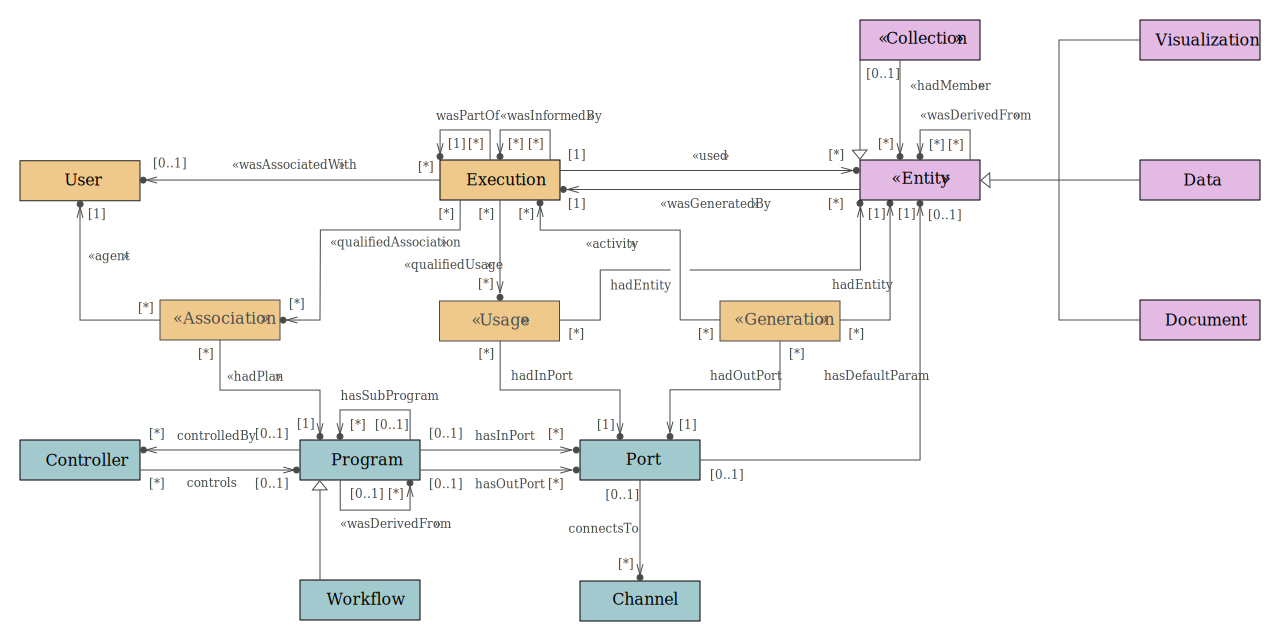
\includegraphics[width=\linewidth]{./provone-model}
\caption{UML depiction of ProvONE}
\label{fig:provone-model}
\end{figure}

\sloppy ProvONE introduces three  commonly used \texttt{prov:Entity} types, namely \texttt{provone:Visualization}, \texttt{provone:Data}, and \texttt{provone:Document}; it also introduces \texttt{provone:User} as a specific type of \texttt{prov:Agent}.
Crucially, ProvONE accounts for a description of static process structure by extending \texttt{prov:Plan} with \texttt{provone:Program} as well as its own extension \texttt{provone:Workflow}, and by introducing new Entity types \texttt{provone:Port} and \texttt{provone:Channel}.
The model is designed to accommodate in particular dataflow-type structures, where Programs have input and output Ports, which are connected by Channels, and Program nesting is expressed using the \texttt{provone:hasSubProgram} relationship.
ProvONE extensions connect to PROV through the \texttt{prov:WasAssociatedWith} relationship, where \texttt{provone:Program} participate as a type of \texttt{prov:Plan}. 

Process execution is described by \texttt{provone:Execution}, an extension of \texttt{prov:Activity} that can participate in \texttt{prov:WasAssociatedWith}, \texttt{prov:Used} and \texttt{prov:WasGeneratedBy} relationships, and also admits a new \texttt{provone:wasPartOf} relationship.

By connecting the \texttt{prov:Plan} extensions with \texttt{provone:Execution}, ProvONE supports rich provenance descriptions where data usage, derivation, and generation are explicitly linked with the programs that produce and consume the data, through observation of data bindings on Program ports and of data flow along Channels.


\section{DataONE support for ProvONE:  infrastructure and tooling}





\bibliography{references}
\bibliographystyle{splncs03}
%\end{small}

\end{document}
